\documentclass[a4paper,10pt]{article}
\usepackage[margin=2.2cm]{geometry}
\usepackage{fontspec}
\setmainfont{TeX Gyre Termes}
\usepackage{booktabs}
\usepackage{amsmath}
\usepackage{pgfplots}
\pgfplotsset{compat=1.18}
\usepackage[hidelinks]{hyperref}
\usepackage{titlesec}
\titleformat{\section}{\normalsize\bfseries}{\thesection}{0.6em}{}
\titlespacing*{\section}{0pt}{1.1em}{0.4em}
\titleformat{\subsection}{\normalsize\itshape}{\thesubsection}{0.6em}{}
\titlespacing*{\subsection}{0pt}{0.7em}{0.2em}
\setlength{\parindent}{0pt}
\setlength{\emergencystretch}{1.5em}
\setlength{\parskip}{0.45em}
\usepackage{caption}
\captionsetup{font=small,labelfont=bf}

\title{\vspace{-1.2cm}\textbf{Song or neighbours? Splitting the Eurovision vote\\ into the entry and the relationship between two countries}}
\author{Anna-Ilona Nikolaeva, Yauheni Zviazdou and Tim Kicker\\
\small Introduction to Data Science, University of Helsinki, October 2026}
\date{}

\begin{document}
\maketitle
\vspace{-1.2em}

\begin{abstract}\small
\noindent
Since 2016 the Eurovision final has reported the jury vote and the public vote of every country separately.
We used this to measure, separately for the juries and the public, how much of a single vote from one country to another comes from the entry itself and how much from the relationship between the two countries.
On finals the models had not seen, the entry alone explains 24.9\,\% of a jury vote and 40.3\,\% of a public vote.
The relationship alone explains 2.8\,\% of a jury vote but 12.5\,\% of a public vote, which means it counts about four times as much for the public.
\end{abstract}

\section{Question and data}

We look at the vote of one country for another in one final, kept apart for jury and public.
The ten finals from 2016 to 2026 (2020 was cancelled) have 260 entries but 19\,800 such votes (about eighty times as many rows) and only with that many rows can the effect of a pair of countries be estimated at all.
The studies of voting bias we know of use the combined points.
None of them keeps jury and public apart, although the rules have allowed it since 2016.
For the forecast we compare with Adamska and Reiss (2025), who report an average rank error of 6.07 for the total score from audio, lyrics and YouTube views while chance lies at 8.55.

\subsection{Data}

Results up to 2023 come from the Eurovision Song Contest Dataset by Spijkervet (2020).
For 2024 to 2026 we read the voting scripts that eurovisionworld.com loads on each results page.
They hold every jury and public point as JSON, so the fetch needs no browser.
Distance, shared border, shared language and colonial ties between two countries come from the GeoDist database of CEPII (Etalab 2.0).
Google Trends interest per voting country (cut on the day before the final) and an automatic analysis of the lyrics come from our teammate repository \texttt{ezvezdov/\allowbreak eurovision-dataset}.
Every download is pinned by its checksum in \texttt{sources.yml} and each run writes down where its files came from.

\subsection{Features}

The models see four kinds of features.
The pair features describe how close two countries are, by the log distance between them, a shared border and a shared official or ethnic language.
Others describe a shared past (a colonial tie, a common coloniser, having once been the same country).
To these we add the mean points the voter gave the receiver in earlier finals and how often the two had met before.
Attention is the search interest for the entry in the voting country, on the web and on YouTube, as Google Trends reports it.
Two features belong to the entry and are the same for every voter, the lyrics (sentiment, theme and repetition) and the running order.
The fourth kind is the receiver effect, the mean of what all other countries gave the same entry.
It stands in for the song but it also carries part of the result we want to predict, which is why we use it to explain votes and never in a forecast.

\section{Method}

\subsection{Validation}

Every model was trained on nine finals and scored on the tenth, once for each year.
The votes within one final depend on each other, so a random split would let the model see part of the year it is tested on.
Everything learned from data comes from the training years, even the median we use to fill missing values.
A test in the code changes the points of one year and checks that the prediction for that year stays the same.

\subsection{Splitting a vote}

For the split we fitted three models per vote type on the points of single votes.
One sees only the entry (the receiver effect), one only the relationship (the pair features) and one sees both.
We measured $R^2$ on the year left out.
The part only the entry explains is then $R^2_{\text{both}}-R^2_{\text{pair}}$ and the part only the relationship explains is $R^2_{\text{both}}-R^2_{\text{entry}}$.
What both explain together is $R^2_{\text{entry}}+R^2_{\text{pair}}-R^2_{\text{both}}$ and whatever is left is noise.
The numbers we report come from ridge regression.
Gradient boosting with a large minimum leaf size served only as a check, because with its default settings boosting learns a pattern that comes from how the receiver effect is built.
The receiver effect leaves out the voter and is therefore slightly different for each voter of the same entry.
Default boosting fits that sawtooth instead of the song.

\subsection{Who favours whom}

To see who favours whom we took the residual of the entry-only model.
It is what a voter gave beyond what the entry earned from everybody else and we averaged it over all finals the two countries shared.
Only pairs that met in at least three finals are listed.

\subsection{Forecast}

For the forecast we compared ridge, gradient boosting and random forest on five sets of features.
We measure the rank error (the mean distance between the predicted and the actual place) against a chance baseline from simulation.
Semi-final results stay out because they are published only after the final.

\section{Results}
\label{sec:results}

\begin{figure}[t]
\centering
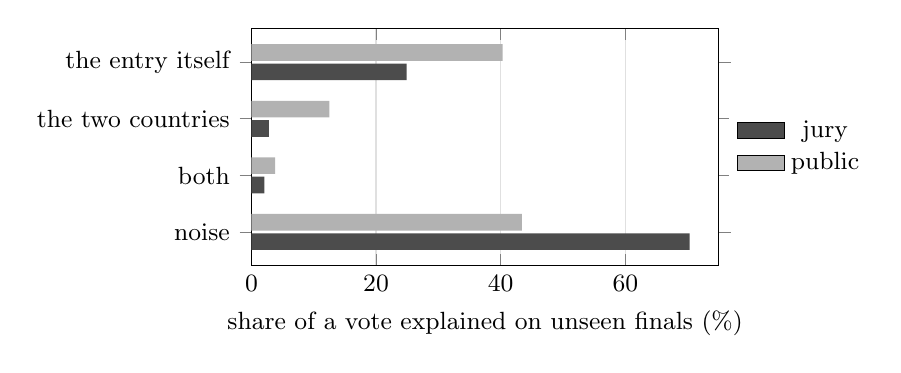
\begin{tikzpicture}
\begin{axis}[
  xbar, width=0.62\textwidth, height=4.6cm, bar width=6pt,
  xmin=0, xmax=75, area legend, xlabel={share of a vote explained on unseen finals (\%)},
  ytick={0,1,2,3}, yticklabels={noise,both,{the two countries},{the entry itself}},
  y dir=normal, ymin=-0.6, ymax=3.6, enlarge y limits=false,
  legend style={at={(1.02,0.5)},anchor=west,draw=none,font=\small},
  tick label style={font=\small}, label style={font=\small},
  xmajorgrids, major grid style={black!12},
]
\addplot[fill=black!70,draw=none,bar shift=-3.5pt] coordinates {(24.9,3) (2.8,2) (2.1,1) (70.3,0)};
\addplot[fill=black!30,draw=none,bar shift=3.5pt] coordinates {(40.3,3) (12.5,2) (3.8,1) (43.4,0)};
\legend{jury,public}
\end{axis}
\end{tikzpicture}
\caption{How much of a vote each part explains, ridge regression on all ten finals. \emph{Both} is what the entry and the relationship explain together. Source: \texttt{decomposition.parquet}.}
\label{fig:split}
\end{figure}

\subsection{Explained shares}

Figure~\ref{fig:split} shows the split.
Measured with ridge the relationship counts 4.5 times as much for the public as for the juries and the boosting check with its large leaf size gives 4.2.
The gap also holds in every single year, since the relationship share lies between 1.5 and 3.9\,\% for the juries and between 5.5 and 18\,\% for the public.
The entry share is probably too high and the relationship share too low, because the receiver effect also carries the bloc votes of all other countries.
Most of a jury vote stays unexplained (70.3\,\%), against 43.4\,\% of a public vote.
All of these shares are about the single vote from one country to another and they say nothing about who wins.

\subsection{Juries and the public}

Juries and the public often disagree.
Over the 257 entries their totals correlate at 0.43 (Spearman).
Israel got 52 points from the juries in 2024 and 323 from the public, while Switzerland got 214 from the juries in 2025 and none at all from the public.
Neighbours are 7.4\,\% of all pairs, yet a neighbour gets one in four of the public's twelve points (25.9\,\%, 396 votes) and only 14.8\,\% of the jury's (393 votes).

\begin{figure}[t]
\centering
\begin{tikzpicture}
\begin{axis}[
  width=0.62\textwidth, height=0.62\textwidth, xmin=0, xmax=520, ymin=0, ymax=520,
  xlabel={points from the juries}, ylabel={points from the public},
  tick label style={font=\small}, label style={font=\small},
  ymajorgrids, major grid style={black!12},
]
\addplot[only marks, mark=o, mark size=1.6pt, draw=black!55] table[col sep=comma,x=jury,y=televote] {../data/export/latex/scatter.csv};
\addplot[dashed, black!40, no marks] coordinates {(0,0) (520,520)};
\addplot[only marks, mark=*, mark size=2pt, black] table[col sep=comma,x=jury,y=televote] {../data/export/latex/scatter-named.csv};
% label positions, the points themselves come from scatter-named.csv
\node[font=\scriptsize,anchor=west] at (axis cs:60,323) {Israel 2024};
\node[font=\scriptsize,anchor=west] at (axis cs:48,291) {Norway 2019};
\node[font=\scriptsize,anchor=west] at (axis cs:200,439) {Ukraine 2022};
\node[font=\scriptsize,anchor=west] at (axis cs:262,36) {Sweden 2018};
\node[font=\scriptsize,anchor=west] at (axis cs:224,12) {Switzerland 2025};
\end{axis}
\end{tikzpicture}
\caption{All 257 finalists since 2016. The dashed line marks the same score from both. Source: \texttt{scatter.csv}.}
\label{fig:scatter}
\end{figure}

\subsection{Who favours whom}

Table~\ref{tab:affinity} lists the pairs that gave each other the most beyond what the entry earned, among pairs that met at least three times.
The Greek public gave Cyprus its twelve points in all eight finals both countries reached and Cyprus did the same for Greece in six of seven.
These numbers cannot tell diaspora, a shared music market, language and politics apart.
With only three meetings a value near $+10$ means three twelves, which is why we read the list as a place to start looking.

\begin{table}[t]
\centering\small
\begin{tabular}{@{}lrrlrr@{}}
\toprule
\multicolumn{3}{c}{Public} & \multicolumn{3}{c}{Juries}\\
\cmidrule(r){1-3}\cmidrule(l){4-6}
Pair & Meetings & Excess & Pair & Meetings & Excess\\
\midrule
Greece $\to$ Cyprus & 8 & +10.5 & Montenegro $\to$ Serbia & 5 & +9.8\\
N. Macedonia $\to$ Albania & 3 & +10.4 & Cyprus $\to$ Greece & 7 & +9.4\\
Cyprus $\to$ Greece & 7 & +9.8 & Azerbaijan $\to$ Russia & 3 & +9.2\\
Georgia $\to$ Armenia & 6 & +9.8 & Greece $\to$ Cyprus & 8 & +8.7\\
Montenegro $\to$ Serbia & 5 & +9.8 & Montenegro $\to$ Albania & 4 & +7.9\\
\bottomrule
\end{tabular}
\caption{Points a country gave beyond what the entry earned from everybody else, averaged over the finals both countries reached. Source: \texttt{pair\_affinity.parquet}.}
\label{tab:affinity}
\end{table}

\subsection{Forecast}

Table~\ref{tab:forecast} gives the rank error on finals the model had not seen, using only data that exists on the day before the final.
With pair features and Google Trends the forecast for the public is off by 5.6 places on average, which is below the 6.07 that Adamska and Reiss report.
Their number is for the total score and ours for the public vote alone, so the two are not directly comparable.
Trends help the forecast for the public about twice as much as the one for the juries.
The lyrics and the running order made the trees worse in every combination we tried.
Both have the same value for every voter of an entry, which lets a tree recognise and memorise the training entries.
Random forest and boosting end up within 0.2 places of each other.
We do not report win probabilities, because the best forecast is badly calibrated and entries it gave more than a 0.5 chance of winning won only one time in eight.

\begin{table}[t]
\centering\small
\begin{tabular}{@{}llcccc@{}}
\toprule
 & & \multicolumn{2}{c}{Jury} & \multicolumn{2}{c}{Public}\\
\cmidrule(r){3-4}\cmidrule(l){5-6}
Features & Model & $\rho$ & Rank error & $\rho$ & Rank error\\
\midrule
chance & & & 8.5 & & 8.4\\
pair & boosting & 0.32 & 6.8 & 0.37 & 6.4\\
pair + lyrics & boosting & 0.21 & 7.5 & 0.29 & 6.8\\
pair + order & boosting & 0.26 & 7.2 & 0.25 & 7.3\\
pair + trends & boosting & 0.39 & 6.4 & 0.51 & 5.6\\
pair + trends & forest & 0.39 & 6.4 & 0.48 & 5.7\\
\bottomrule
\end{tabular}
\caption{Forecast on the year left out, with Spearman's $\rho$ between predicted and actual place and the mean rank error. Source: \texttt{model\_summary.parquet}.}
\label{tab:forecast}
\end{table}

\section{Limits}

Ten finals are a small sample and the yearly ranges in Section~\ref{sec:results} show how much one final can move a share.
The public vote of the rest of the world (counted since 2023) is a single pooled voter without geography, so we left it out of the pair statistics.
Google Trends samples its series and Bosnia is missing from the Trends list, which leaves 52 panel rows without a Trends value.

The relationship features describe two countries but they do not show why a voter gives points.
A shared border and a shared language usually come together with large diasporas and the model cannot pull them apart.
The receiver effect only knows the song through what other countries gave it, so the entry share includes bloc votes and cannot tell a good song from a popular one.
What the split measures is explained variance on years the model did not see, which says nothing about whether any single vote was influenced.

We left out the age and sex of the artists.
A third of the entries are bands that have neither value and matching names would have cost hours for an entry feature that would probably not have helped the trees either, given what the lyrics and the running order did.

\section{Reproducibility}

The code is available to the course staff on request.
We ran the whole pipeline with one command (\texttt{uv run esc all}, which fetches and parses the data, builds the panel and fits the models) on Linux and on a Windows laptop and got the same results both times.
Since the sources are pinned by checksum and the seed is fixed at 20260501, two runs on the same inputs produce identical tables.
All 82 tests run offline and pass on Linux.

\medskip
\footnotesize
\textbf{References.}
Adamska, J. and Reiss, J. D. (2025). \emph{Transactions of the International Society for Music Information Retrieval} 8(1), 93--107.
Spijkervet, J. (2020). The Eurovision Song Contest Dataset. Zenodo, doi:10.5281/zenodo.4036457.
Mayer, T. and Zignago, S. (2011). Notes on CEPII's distance measures: the GeoDist database. CEPII Working Paper 2011-25.

\section*{Appendix: features and settings}

\small
The panel has a row for every vote one country gave another in a final, separately for jury and public, which makes 19\,800 rows.
A pair where the voter gave nothing keeps zero points, because only ten countries score in each vote and dropping the zeros would leave a panel made of successes only.
Votes from a country to itself are dropped and so is the pooled public vote of the rest of the world, since it has no geography.
Table~\ref{tab:features} lists the features.

\begin{table}[h]
\centering\small
\begin{tabular}{@{}ll@{}}
\toprule
Feature & Meaning\\
\midrule
\texttt{log\_dist} & log of the distance between the two countries (CEPII)\\
\texttt{contig}, \texttt{smctry} & shared border, same country (CEPII)\\
\texttt{comlang\_off}, \texttt{comlang\_ethno} & shared official or ethnic language (CEPII)\\
\texttt{colony}, \texttt{comcol} & colonial tie, common coloniser (CEPII)\\
\texttt{past\_points}, \texttt{past\_meetings} & mean points the voter gave the receiver in earlier finals, number of earlier finals\\
\texttt{web\_interest}, \texttt{youtube\_interest} & Google Trends interest for the entry in the voting country, cut the day before the final\\
\texttt{running\_position} & running order scaled to $[0,1]$\\
lyrics & sentiment, theme, repetition in verse and chorus (automatic analysis)\\
\texttt{receiver\_effect} & mean of what all other voters gave the same entry, explanatory only\\
\bottomrule
\end{tabular}

\caption{Features in the panel.}
\label{tab:features}
\end{table}

The set called \emph{pair} uses the first nine features in the table.
The other sets add the lyrics, the running order, the two Trends series or Trends and running order together.
A set with the receiver effect counts as explanatory and its results are never reported as a forecast.

Ridge regression picked its penalty from 13 values between $10^{-3}$ and $10^{3}$ by leave-one-out cross-validation on the training rows.
For gradient boosting we used the histogram version with depth 4, a learning rate of 0.06 and 300 iterations.
In the decomposition it also had a minimum leaf size of 200.
The random forest had 200 trees with a minimum leaf size of 20 and looked at half of the features at each split.
Missing values were filled with the median of the training years.
The chance baseline uses the seed 20260501 and the models use 0.

Each year was held out as a whole, which means the model was fitted on the pair rows of the other nine finals and predicted the rows of the held-out one.
We summed the predicted points per entry, turned the sums into places and compared those with the actual places in that final.
The rank error is the mean absolute difference between predicted and actual place, averaged over the finals.
For the chance baseline we shuffled the actual places within each final 1\,000 times, which gives a mean of 8.5 for the juries and 8.4 for the public.

\end{document}
